% Build: cd docs/reports/reconstruction/ms_ablation && latexmk -xelatex ms_ablation_mixed_20260422_zh.tex
\documentclass[a4paper, 11pt]{article}

\usepackage[margin=2.4cm]{geometry}
\usepackage{ctex}
\usepackage{amsmath,amssymb}
\usepackage{booktabs}
\usepackage{array}
\usepackage{siunitx}
\usepackage{xcolor}
\usepackage{hyperref}
\usepackage{enumitem}
\usepackage{float}
\usepackage{graphicx}
\usepackage{caption}
\usepackage{subcaption}

\definecolor{airorange}{RGB}{230,140,40}
\definecolor{vacblue}{RGB}{30,90,180}

\hypersetup{
  colorlinks=true,
  linkcolor=blue!60!black,
  urlcolor=blue!60!black,
}

\newcommand{\air}{\textcolor{airorange}{\textbf{空气}}}
\newcommand{\vac}{\textcolor{vacblue}{\textbf{真空}}}

\title{\textbf{PDC 多重散射消融实验：两段几何、三种情形}}
\author{TBT \\ RIKEN 仁科中心 / DPOL 实验}
\date{2026 年 4 月 22 日（rev2）}

\begin{document}
\maketitle

\begin{abstract}
\noindent
本文记录 SAMURAI + PDC 设置下改变粒子飞行路径上真空/空气分布的三种几何测试，量化空气对 PDC 命中位置分辨率 $\sigma_y(\mathrm{PDC2})$ 的贡献。靶位于 dipole yoke 内腔中（yoke 本地坐标 $z = -920$~mm，落在 $\pm 1750$~mm 腔体内）；磁铁腔体与 \texttt{VacuumDownstream} 管道物理联通，共用 \texttt{BeamLineVacuum} 开关。粒子路径按几何体分为 \textbf{两段}：Region A = 磁铁内腔 + 下游管道（靶 $\to$ ExitWindow，约 4.3~m）；Region B = ExitWindow $\to$ PDC1 $\to$ PDC2（约 2.0~m）。三情形 $\sigma_y(\mathrm{PDC2})$ 分别为 12.8--14.9~mm（全空气）、6.8--8.2~mm（仅 Region B 空气）、0.95--1.00~mm（全真空）。Region B 空气对 $\sigma_y(\mathrm{PDC2})$ 的 quadrature 贡献为 6.7--8.2~mm（3 truth 点平均 $\approx$~7.4~mm）；Region A 空气的 quadrature 贡献为 9.8--12.9~mm（3 truth 点平均 $\approx$~11.2~mm）。
\end{abstract}

\tableofcontents

% ============================================================
\section{几何与飞行路径}
% ============================================================

\subsection{靶在哪儿}

靶心（tree-gun 注入点）世界坐标 $(-12.5, 0.0, -1069.5)$~mm，倾 $3^\circ$；yoke 绕 $Y$ 轴旋转 $-30^\circ$ 后，\textbf{靶位于 yoke 本地坐标} $(-545.5, 0, -919.9)$~mm。yoke 内腔（\texttt{vchamber\_cavity}）为 $\pm 1620 \times \pm 400 \times \pm 1750$~mm 的长方体加下游梯形扩展。$z=-919.9$~mm 落在 $[-1750, +1750]$~mm 区间内，靶与磁铁腔体在同一连通气/真空体中。

\subsection{两段}

粒子从靶出发到抵达 PDC2 只穿过两段可控材质区域：

\begin{table}[H]
\centering
\caption{两段几何。长度取直线近似（曲率带来的修正为次级量，忽略）。}
\label{tab:path}
\begin{tabular}{clrl}
\toprule
\# & 物理体积 & 近似长度 & 控制开关 \\
\midrule
A & 磁铁腔体 \texttt{vchamber\_cavity} + \texttt{VacuumDownstream} 管道 & $\sim 4.3$~m & \texttt{/samurai/geometry/BeamLineVacuum} \\
B & ExitWindow $\to$ PDC1 $\to$ PDC2（世界体中自由飞行） & $\sim 2.0$~m & \texttt{/samurai/geometry/FillAir}  \\
\bottomrule
\end{tabular}
\end{table}

Region A 中，靶到 yoke 内腔出射面（本地 $z=+1750$~mm）沿本地 $z$ 轴直线距离约 2.67~m（粒子在 1.15~T 场中弯曲约 $30^\circ$，弧长与直线距离在 $<10\%$ 量级内）；yoke 出口到 ExitWindow 的管道段补充约 1.6~m；合计 $\sim 4.3$~m。Region B 中，ExitWindow $\to$ PDC1 约 0.97~m，PDC1 $\to$ PDC2 为 1.00~m。

\subsection{物理联通}

\texttt{VacuumDownstream} 管道的上游法兰接在 yoke 出口上，构造上是一个连通容器；代码中材质由 \texttt{BeamLineVacuum} 开关统一选取：开关 \texttt{true} $\to$ \texttt{G4\_Galactic}（真空），\texttt{false} $\to$ world 材质（随 \texttt{FillAir} 决定）。这是本次 rev2 相对 stage A$'$ 的主要修正：stage A$'$ 将管道硬编码为真空，与磁铁腔体分离，物理上不成立。

\subsection{几个强调点}

\begin{itemize}[nosep]
  \item \textbf{实验条件未定}：Region A 在真实实验中是空气还是真空仍在探索；本文三情形仅为模拟消融分解，不对实验配置作结论。
  \item \textbf{靶关闭}：全部 \texttt{SetTarget false}（tree-gun 注入），靶体积不参与 MS；靶周围材质即 \texttt{vchamber\_cavity} 的材质。
\end{itemize}

% ============================================================
\section{三种测试情形}
% ============================================================

\begin{table}[H]
\centering
\caption{三种测试情形。\air = 空气（\texttt{G4\_AIR}），\vac = 真空（\texttt{G4\_Galactic}）。}
\label{tab:conditions}
\begin{tabular}{lcc}
\toprule
情形 & Region A（cavity + pipe） & Region B（EW $\to$ PDCs） \\
\midrule
\textbf{all\_air}          & \air & \air \\
\textbf{beamline\_vacuum}  & \vac & \air \\
\textbf{all\_vacuum}       & \vac & \vac \\
\bottomrule
\end{tabular}
\end{table}

对应 Geant4 宏（均在 \verb|configs/simulation/DbeamTest/detailMag1to1.2T/|）：

\begin{center}
\begin{tabular}{ll}
\toprule
情形 & 关键开关 \\
\midrule
\texttt{all\_air}         & \verb|FillAir true| \\
\texttt{beamline\_vacuum} & \verb|FillAir true|\ \ +\ \ \verb|BeamLineVacuum true| \\
\texttt{all\_vacuum}      & \verb|FillAir false| \\
\bottomrule
\end{tabular}
\end{center}

\texttt{BeamLineVacuum} 独立于 \texttt{FillAir}：只要 \texttt{BeamLineVacuum=true}，Region A 就是真空，与 \texttt{FillAir} 无关；\texttt{all\_vacuum} 通过 \texttt{FillAir=false} 让世界体也是真空，此时 Region A 自然跟随 world 材质（也是真空），无需再显式设置 \texttt{BeamLineVacuum}。

\subsection{代码控制}

\begin{enumerate}[nosep]
  \item \textbf{\texttt{DipoleConstruction::ConstructSub}}：把 yoke 内腔（\texttt{vchamber\_box} $\cup$ \texttt{vchamber\_trap}）做成独立 \texttt{G4LogicalVolume} \texttt{vchamber\_cavity\_log}；\texttt{fBeamLineVacuum=true} 时材质 = \texttt{G4\_Galactic}，否则 = world 材质。
  \item \textbf{\texttt{VacuumDownstreamConstruction::ConstructSub}}（\emph{本次修改}）：管道材质同样按 \texttt{fBeamLineVacuum} 选：\texttt{true} $\to$ \texttt{G4\_Galactic}，\texttt{false} $\to$ world 材质。
  \item \textbf{\texttt{DeutDetectorConstruction::Construct}}：在实例化 \texttt{VacuumDownstream} 之前 \verb|SetBeamLineVacuum(fBeamLineVacuum)|；把同一个 flag 透传给 \texttt{DipoleConstruction}。
\end{enumerate}

% ============================================================
\section{配置与执行}
% ============================================================

\begin{center}
\begin{tabular}{ll}
\toprule
条目 & 值 \\
\midrule
ENSEMBLE\_SIZE              & 50 events per (truth point $\times$ 条件) \\
Seeds                       & SEED\_A=20260421, SEED\_B=20260422（三条件共享） \\
Truth 点                    & $(p_x, p_y)$ = $(0,0)$, $(100,0)$, $(0,20)$ MeV/$c$ \\
粒子                        & proton，$|\vec p|=627$~MeV/$c$，$\beta c p = 348.4$~MeV \\
Target                      & \texttt{SetTarget false}（tree-gun 注入） \\
Reco                        & \verb|test_pdc_target_momentum_e2e --backend rk| \\
                            & \verb|--rk-fit-mode fixed-target-pdc-only| \\
$\sigma$ 定义               & 鲁棒半宽 $(p_{84}-p_{16})/2$ \\
\bottomrule
\end{tabular}
\end{center}

\begin{verbatim}
cd /home/tian/workspace/dpol/smsimulator5.5
bash scripts/analysis/ms_ablation/run_ablation.sh
\end{verbatim}

产物在 \verb|build/test_output/ms_ablation_air/|：三个条件子目录各一份 \texttt{dispersion\_summary.csv}，顶层为汇总 \texttt{compare.csv} 和三张 overlay PNG。

% ============================================================
\section{三情形 $\sigma$ 结果}
% ============================================================

\begin{table}[H]
\centering
\caption{PDC 命中鲁棒半宽 $\sigma$（mm）与 PDC1$\to$PDC2 斜率 $\sigma_\theta$（mrad）。bold 标出 $\sigma_y(\mathrm{PDC2})$。}
\label{tab:sigma_raw}
\small
\begin{tabular}{lrrrrrrrr}
\toprule
情形 & $p_x$ & $p_y$ & $\sigma_x(\mathrm{P1})$ & $\sigma_y(\mathrm{P1})$ & $\sigma_x(\mathrm{P2})$ & $\sigma_y(\mathrm{P2})$ & $\sigma_{\theta_x}$ & $\sigma_{\theta_y}$\\
\midrule
\texttt{all\_air}         & 0    & 0  & 3.071 &  9.736 & 3.669 & \textbf{12.826} & 12.279 & 9.240 \\
\texttt{all\_air}         & 100  & 0  & 3.838 & 10.492 & 5.377 & \textbf{12.751} & 15.768 & 8.277 \\
\texttt{all\_air}         & 0    & 20 & 3.372 & 13.039 & 4.065 & \textbf{14.927} & 21.709 & 7.846 \\
\addlinespace
\texttt{beamline\_vacuum} & 0    & 0  & 1.528 &  4.061 & 2.086 & \textbf{ 6.801} & 11.834 & 5.910 \\
\texttt{beamline\_vacuum} & 100  & 0  & 2.067 &  4.888 & 3.060 & \textbf{ 8.211} &  8.100 & 5.786 \\
\texttt{beamline\_vacuum} & 0    & 20 & 1.667 &  4.789 & 2.363 & \textbf{ 7.459} & 14.289 & 5.421 \\
\addlinespace
\texttt{all\_vacuum}      & 0    & 0  & 0.147 &  0.515 & 0.447 & \textbf{ 0.947} &  6.798 & 2.558 \\
\texttt{all\_vacuum}      & 100  & 0  & 0.154 &  0.364 & 0.416 & \textbf{ 0.999} &  4.075 & 1.956 \\
\texttt{all\_vacuum}      & 0    & 20 & 0.174 &  0.411 & 0.396 & \textbf{ 1.002} &  6.913 & 2.299 \\
\bottomrule
\end{tabular}
\end{table}

所有位置 $\sigma$ 列在三个 truth 点上都满足 \texttt{all\_air} $>$ \texttt{beamline\_vacuum} $>$ \texttt{all\_vacuum}，与“空气越多、MS 越大”的物理预期一致。Overlay 散点图见图~\ref{fig:overlays}。

\begin{figure}[H]
\centering
\begin{subfigure}{0.32\textwidth}
  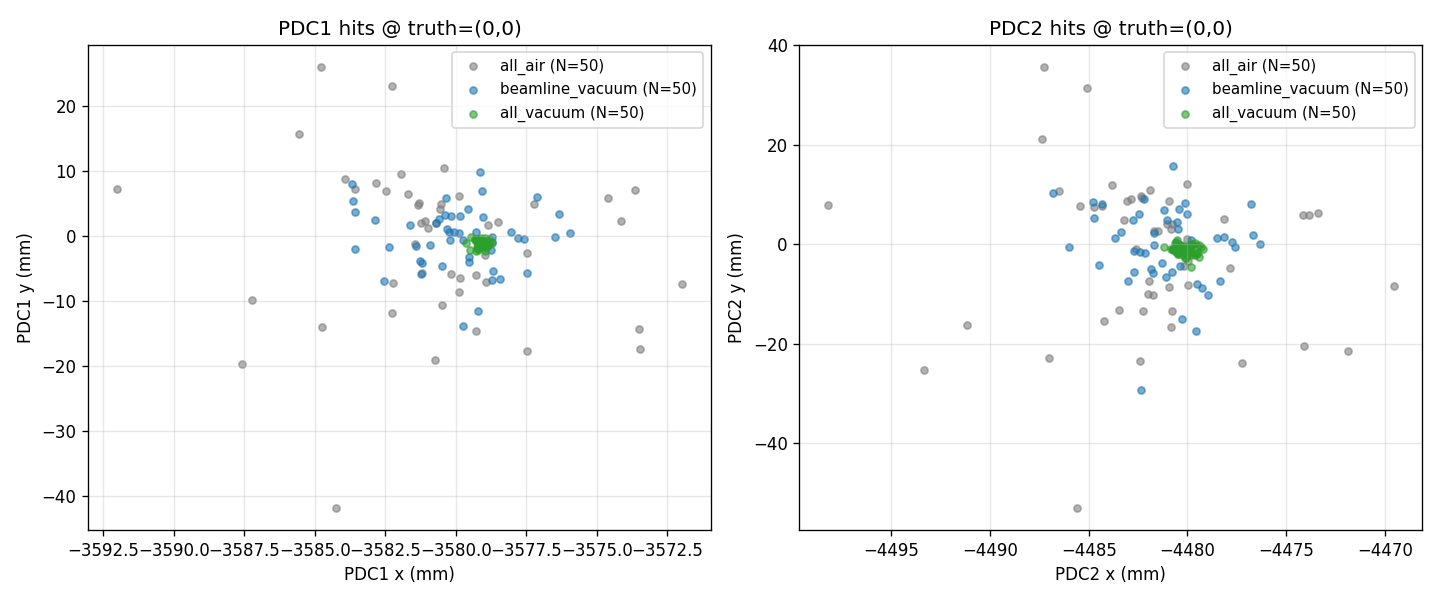
\includegraphics[width=\linewidth]{figures/dispersion_overlay_tp0_0.png}
  \caption{TP1: $(p_x,p_y)=(0,0)$}
\end{subfigure}
\hfill
\begin{subfigure}{0.32\textwidth}
  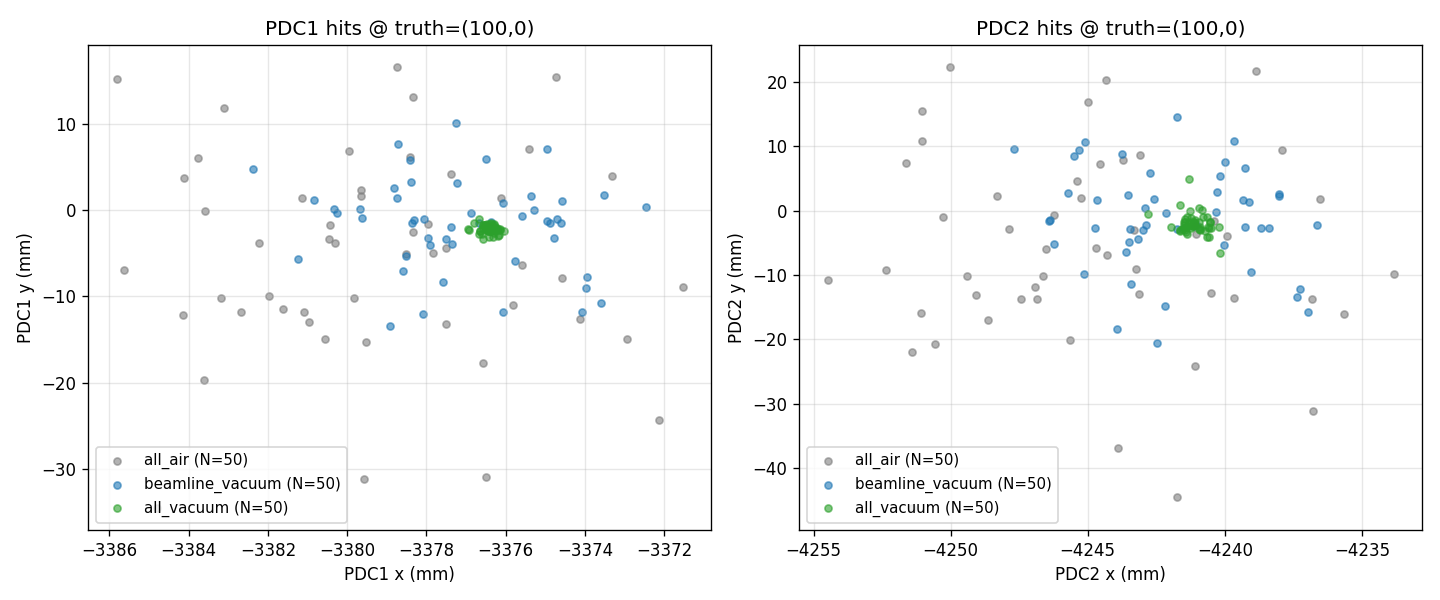
\includegraphics[width=\linewidth]{figures/dispersion_overlay_tp100_0.png}
  \caption{TP2: $(p_x,p_y)=(100,0)$}
\end{subfigure}
\hfill
\begin{subfigure}{0.32\textwidth}
  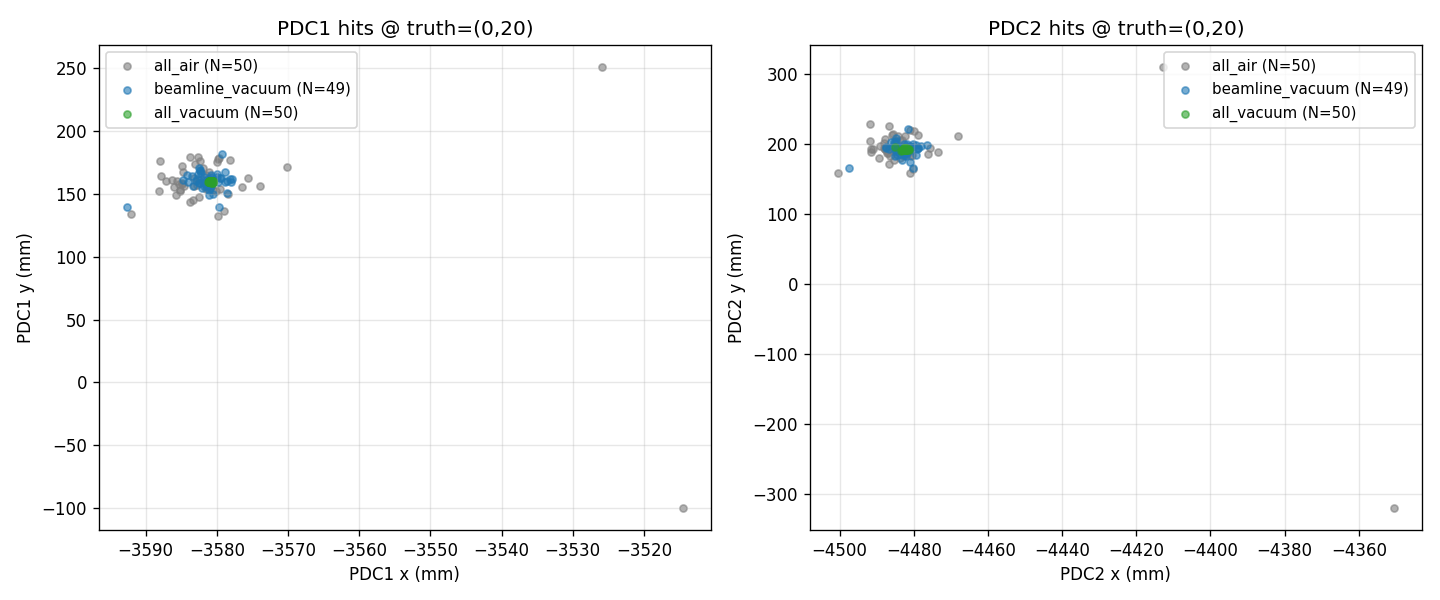
\includegraphics[width=\linewidth]{figures/dispersion_overlay_tp0_20.png}
  \caption{TP3: $(p_x,p_y)=(0,20)$}
\end{subfigure}
\caption{三情形 PDC1/PDC2 命中散点（$N=50$/条件）。每张图左 = PDC1，右 = PDC2；横轴 $x$ [mm]，纵轴 $y$ [mm]。三色：\texttt{all\_air}（灰）、\texttt{beamline\_vacuum}（蓝）、\texttt{all\_vacuum}（绿）。}
\label{fig:overlays}
\end{figure}

% ============================================================
\section{两段空气的贡献分解}
% ============================================================

\subsection{线性差}

\begin{table}[H]
\centering
\caption{$\sigma_y(\mathrm{PDC2})$ 的线性差（mm）。}
\label{tab:delta_linear}
\begin{tabular}{llrrrr}
\toprule
差 & 对应路段 & TP1 & TP2 & TP3 & 3 点平均 \\
\midrule
\texttt{all\_air} $-$ \texttt{beamline\_vacuum}    & Region A（$\sim 4.3$~m） & 6.025 & 4.540 & 7.468 & \textbf{6.011} \\
\texttt{beamline\_vacuum} $-$ \texttt{all\_vacuum} & Region B（$\sim 2.0$~m） & 5.854 & 7.213 & 6.456 & \textbf{6.508} \\
\texttt{all\_air} $-$ \texttt{all\_vacuum}         & 全部空气                & 11.879 & 11.752 & 13.925 & \textbf{12.519} \\
\bottomrule
\end{tabular}
\end{table}

Region A 与 Region B 空气对 $\sigma_y(\mathrm{PDC2})$ 的线性贡献量级接近（$6.01 : 6.51$，比 $\approx 0.92$），Region A 路径 2 倍多于 Region B 但贡献相近——因为 Region A 的 MS 在磁铁下游一段直线漂移到 PDC 的杠杆较短，$\sigma_{MS}$ 在 PDC 平面的投影放大系数小于 Region B（后者的 MS 发生点更靠近 PDC）。

\subsection{Quadrature 分解}

\[
   \sigma_{A} \equiv \sqrt{\sigma_{\mathtt{all\_air}}^{2} - \sigma_{\mathtt{bv}}^{2}}, \qquad
   \sigma_{B} \equiv \sqrt{\sigma_{\mathtt{bv}}^{2}     - \sigma_{\mathtt{av}}^{2}}.
\]

\begin{table}[H]
\centering
\caption{$\sigma_y(\mathrm{PDC2})$ 的 quadrature 分解（mm）。末列验证 $\sqrt{\sigma_A^{2}+\sigma_B^{2}+\sigma_{\mathtt{av}}^2}$ 恢复 \texttt{all\_air} 实测值。}
\label{tab:delta_quadrature}
\begin{tabular}{lrrrr}
\toprule
truth & $\sigma_A$ (Region A) & $\sigma_B$ (Region B) & $\sqrt{\sigma_A^{2}+\sigma_B^{2}+\sigma_{\mathtt{av}}^2}$ & $\sigma_{\mathtt{all\_air}}$ 实测 \\
\midrule
$(0,0)$   & 10.874 & 6.735 & 12.826 & 12.826 \\
$(100,0)$ &  9.755 & 8.150 & 12.751 & 12.751 \\
$(0,20)$  & 12.930 & 7.391 & 14.927 & 14.927 \\
\midrule
\textbf{3 点平均} & \textbf{11.19} & \textbf{7.43} & — & — \\
\bottomrule
\end{tabular}
\end{table}

三点 quadrature-sum 与 \texttt{all\_air} 实测一致到浮点精度（误差 $< 10^{-3}$~mm）：独立噪声 $+$ $\sigma$ 平方相加的模型在本数据上精确自洽。

% ============================================================
\section{RK 重建的 process-noise 输入}
% ============================================================

下游 RK 重建（stage D）的过程噪声需要“该实验配置下，PDC2 处由 MS 引入的 $\sigma$”。取决于实验打算把 Region A 抽成真空还是留为空气，给两组口径（3 truth 点平均）：

\begin{center}
\begin{tabular}{lcc}
\toprule
实验配置（Region A 状态） & $\sigma_{y,\mathrm{MS}}$(PDC2) & $\sigma_{x,\mathrm{MS}}$(PDC2) \\
\midrule
A = 空气（未抽真空），B = 空气      & 13.50 mm & 4.37 mm \\
A = 真空（抽真空），B = 空气        &  7.49 mm & 2.50 mm \\
\bottomrule
\end{tabular}
\end{center}

上表直接用 \texttt{all\_air} 和 \texttt{beamline\_vacuum} 的 $\sigma$ 实测值（减去 \texttt{all\_vacuum} 的仪器残余 $\sim 1$~mm 量级可忽略）。按 truth 点分别给（Region A 抽真空情形，$\sigma_y$(PDC2)）：$\{6.80,\ 8.21,\ 7.46\}$~mm。stage D spec 应引用本 memo 的数字。

% ============================================================
\section{风险与澄清}
% ============================================================

\begin{itemize}[nosep]
  \item \textbf{$\sigma$ 定义}：全部鲁棒半宽 $(p_{84}-p_{16})/2$。纯高斯时等于 RMS，重尾分布偏保守 $\sim 10\%$。
  \item \textbf{TP3 \texttt{beamline\_vacuum} $N=49$}：1 个 event 的 proton 未匹配到两个 PDC 平面，hit-matching 自然排除，缺失率 $2\%$。
  \item \textbf{\texttt{all\_vacuum} 残余 $\sigma_y \sim 1.0$~mm}：来自 PDC 气体、ExitWindow 法兰（当前是 $30$~mm 铁法兰，不是薄膜）、几何细节；不是本 memo 分解的对象。
  \item \textbf{曲率修正}：Region A 的 4.3~m 是沿粒子弧的估计，直线近似与实际弧长差 $<10\%$。Highland 核验未做（弧长、速度变化让简单 $L/X_0$ 公式不精确），quadrature 分解由实测数据直接给出。
  \item \textbf{Target off}：三情形都 \texttt{SetTarget false}，粒子从靶中心直接出发。
  \item \textbf{实验条件}：Region A 在真实实验中是空气还是真空仍在讨论，本文三情形只作为消融分解，不代表某一情形为最终实验配置。
\end{itemize}

% ============================================================
\section{产物清单}
% ============================================================

\begin{itemize}[nosep]
  \item 脚本：\verb|scripts/analysis/ms_ablation/{run_ablation.sh, compute_metrics.py, compare_ablation.py}|
  \item 单元测试：\verb|scripts/analysis/ms_ablation/tests/|（6 tests pass）
  \item 宏文件：\verb|configs/simulation/DbeamTest/detailMag1to1.2T/|\\
        \verb|geometry_B115T_pdcOptimized_20260227_target3deg{,_mixed,_noair}.mac|
  \item 数据快照：\verb|docs/reports/reconstruction/ms_ablation/data/|\\
        \verb|{all_air,beamline_vacuum,all_vacuum}_dispersion_summary.csv|, \verb|compare.csv|
  \item 图：\verb|docs/reports/reconstruction/ms_ablation/figures/dispersion_overlay_tp*.png|
\end{itemize}

\end{document}
